\section{Resultados}

\begin{frame}{Modelo sintético Marmousi2}
	\begin{columns}[T]
		\column{0.6\textwidth}
		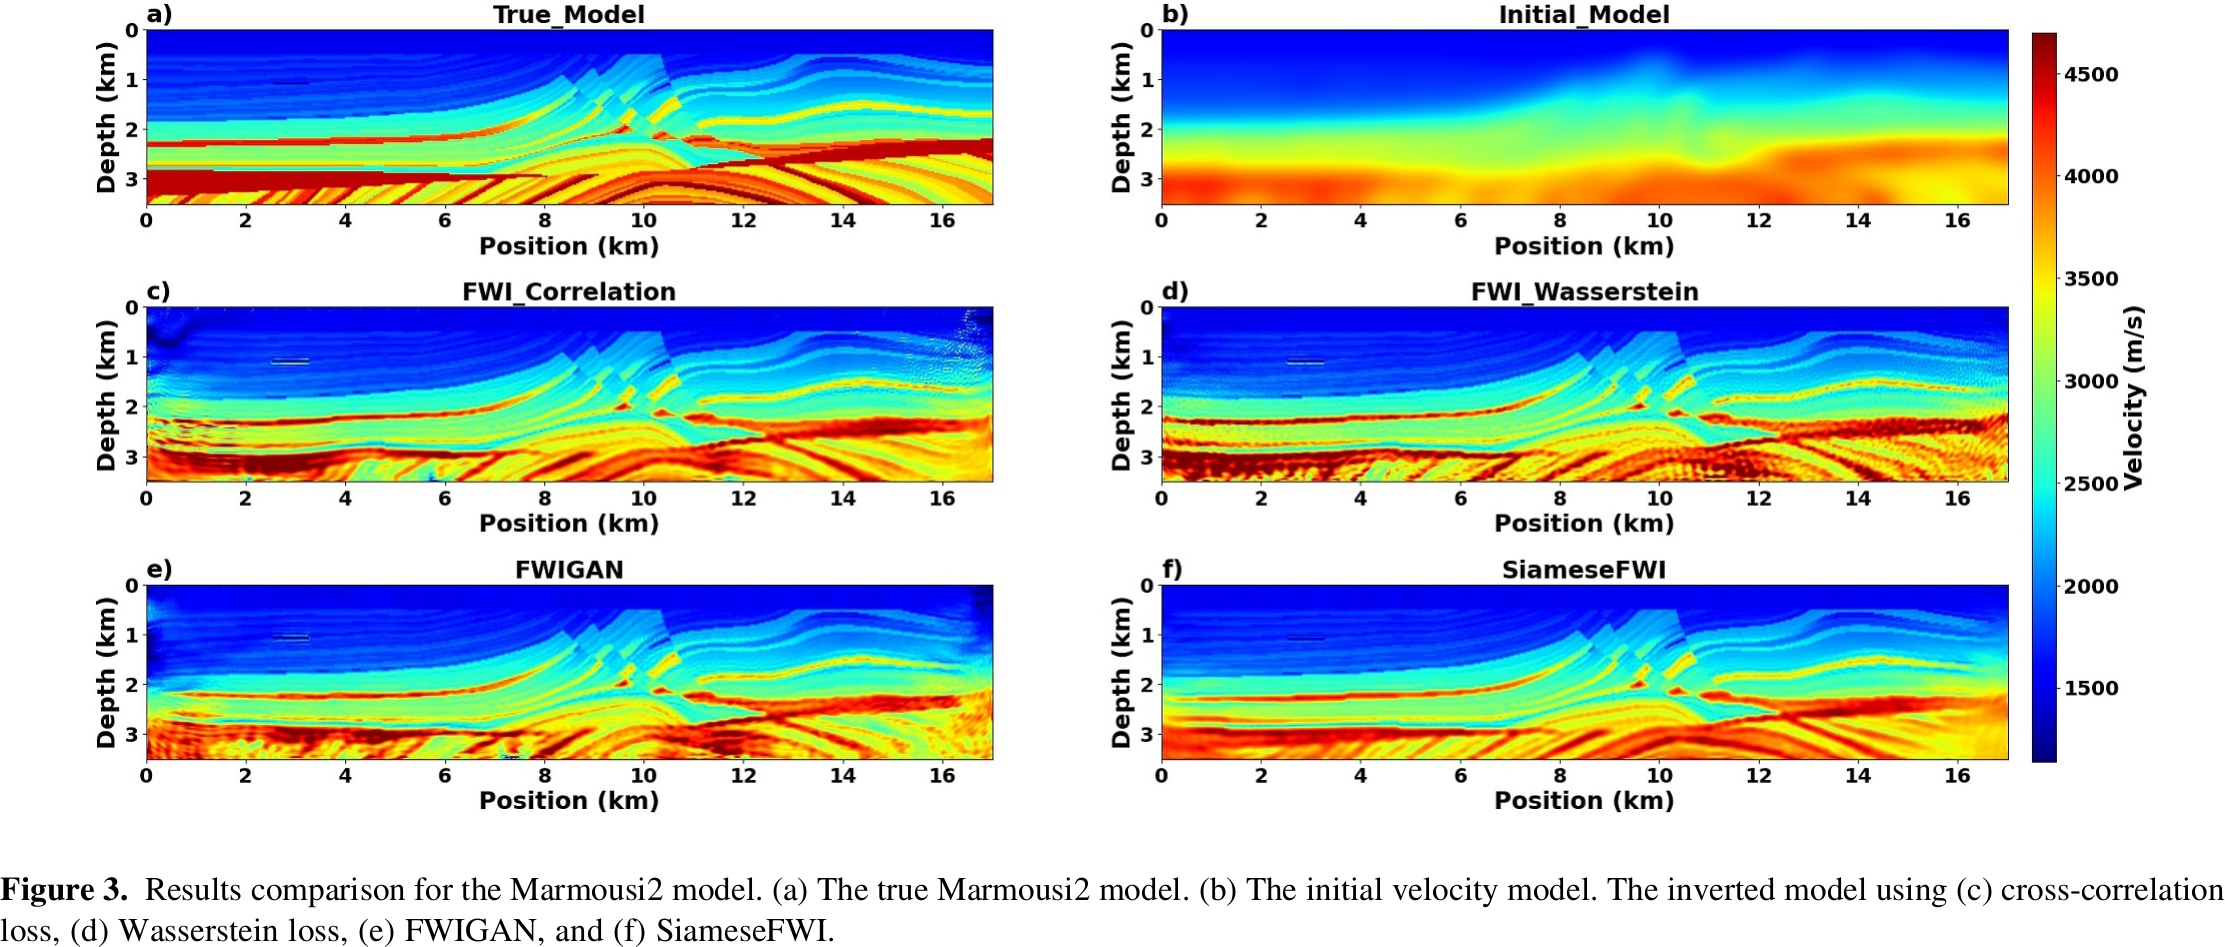
\includegraphics[width=\textwidth]{figuras/paper/fig3_marmousi}
		\column{0.4\textwidth}
		\footnotesize
		\begin{tabular}{lccc}
			\hline
			Método & SNR (dB) & SSIM & RMSE \\
			\hline
			Correlação cruzada & 19,18 & 0,602 & 0,311 \\
			Wasserstein & 19,42 & 0,588 & 0,303 \\
			FWIGAN & 19,06 & 0,583 & 0,316 \\
			\textbf{SiameseFWI} & \textbf{22,57} & \textbf{0,750} & 0,211 \\
			\hline
		\end{tabular}
	\end{columns}
	\vspace{0.2cm}
	\footnotesize SiameseFWI obtém o melhor SNR, SSIM e RMSE entre os quatro métodos, com custo de apenas 10\%--20\% a mais que o FWI convencional.
\end{frame}

\begin{frame}{Modelo sintético Overthrust}
	\begin{columns}[T]
		\column{0.6\textwidth}
		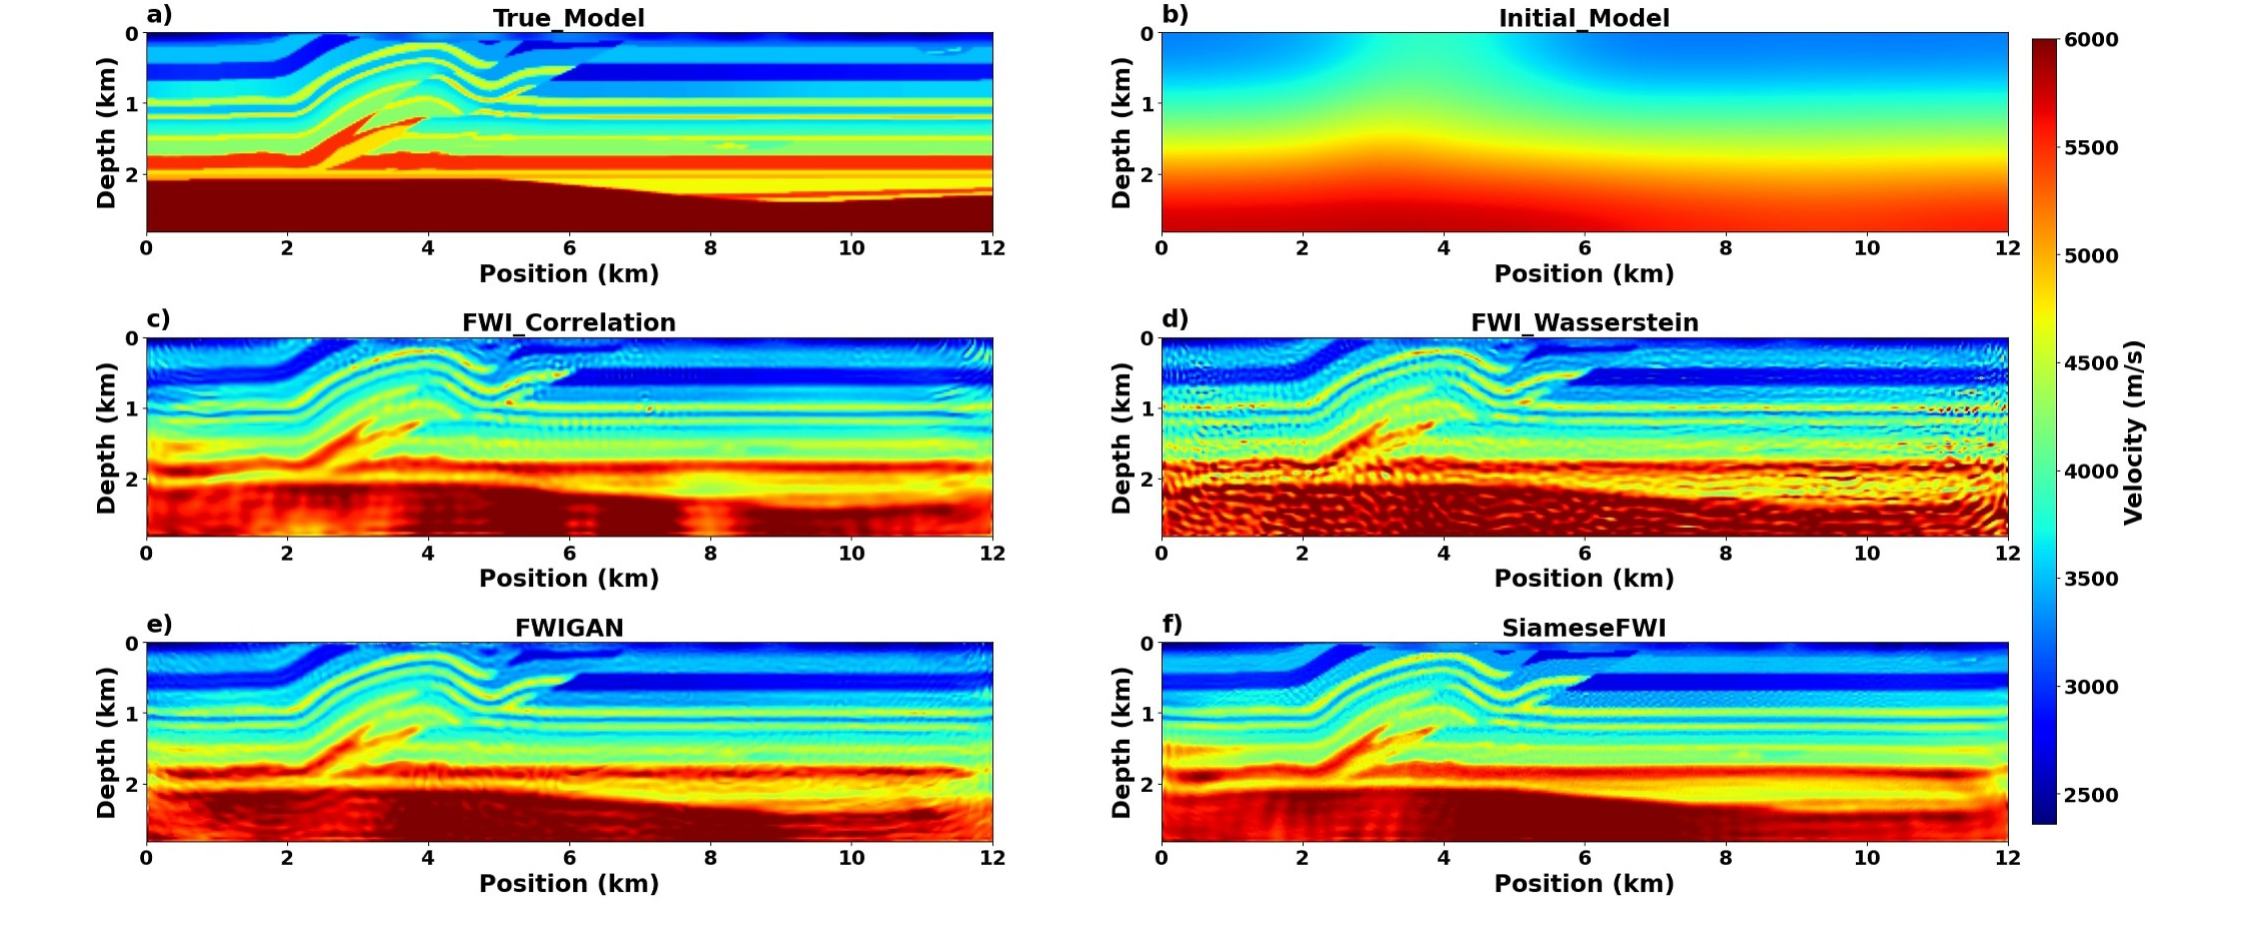
\includegraphics[width=\textwidth]{figuras/paper/fig6_overthrust}
		\column{0.4\textwidth}
		\footnotesize
		\begin{tabular}{lccc}
			\hline
			Método & SNR (dB) & SSIM & RMSE \\
			\hline
			Correlação cruzada & 24,52 & 0,663 & 0,218 \\
			Wasserstein & 23,25 & 0,547 & 0,315 \\
			FWIGAN & 25,95 & 0,663 & 0,228 \\
			\textbf{SiameseFWI} & \textbf{26,98} & \textbf{0,725} & \textbf{0,211} \\
			\hline
		\end{tabular}
	\end{columns}
	\vspace{0.2cm}
	\footnotesize Mesmo padrão do Marmousi2: SiameseFWI à frente em SNR e SSIM, enquanto o FWIGAN (outro método baseado em rede neural) é cerca de 6 vezes mais lento.
\end{frame}

\begin{frame}{Dado de campo (Austrália)}
	\begin{center}
		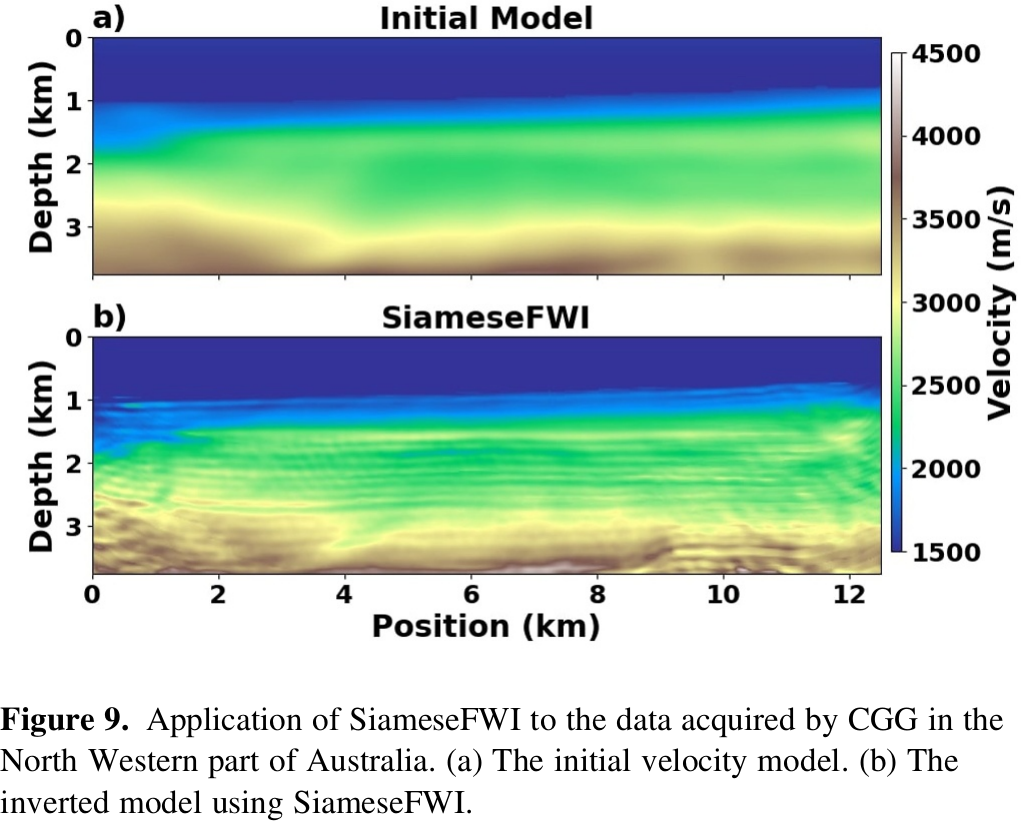
\includegraphics[width=0.34\textwidth]{figuras/paper/fig9_field}
	\end{center}
	\vspace{-0.15cm}
	\begin{itemize}
		\scriptsize
		\setlength{\itemsep}{2pt}
		\item Dado sísmico marinho real, sem modelo de velocidade verdadeiro conhecido.
		\item O modelo invertido pelo SiameseFWI ajusta melhor os dados observados que o modelo inicial, sobretudo nos afastamentos maiores entre fonte e receptor.
		\item Migração reversa no tempo (RTM) com o modelo invertido resolve melhor as interfaces entre 1,5 e 2 km de profundidade.
	\end{itemize}
\end{frame}

\begin{frame}{Robustez do SiameseFWI}
	\begin{itemize}
		\item \textbf{Ruído:} com ruído branco gaussiano aditivo (SNR do dado de $-5$ dB), SiameseFWI mantém SNR de 23,48 dB no modelo invertido, contra 19,18 dB da perda de Wasserstein.
		\item \textbf{Modelo inicial impreciso:} mesmo partindo de um modelo inicial linear (sem nenhuma estrutura real), SiameseFWI converge para um modelo próximo ao verdadeiro.
		\item \textbf{\textit{Wavelet} de fonte desconhecida:} ao estimar a \textit{wavelet} junto com o modelo de velocidade, o método ainda atinge SNR de 24 dB.
	\end{itemize}
\end{frame}
